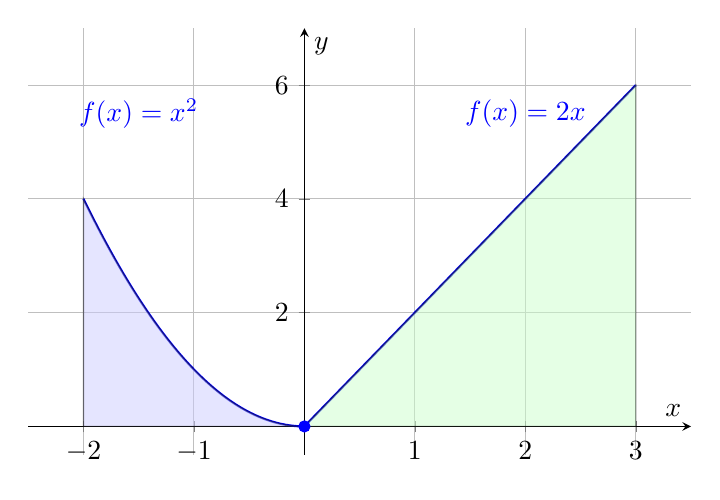
\begin{tikzpicture}
\begin{axis}[
    axis lines=center,
    xlabel=$x$, ylabel=$y$,
    domain=-2.5:3.5,
    samples=100,
    ymin=-0.5, ymax=7,
    xmin=-2.5, xmax=3.5,
    width=10cm, height=7cm,
    xtick={-2,-1,0,1,2,3},
    ytick={0,2,4,6},
    grid=major
]
% Piecewise function: f(x) = x^2 for x <= 0, 2x for x > 0
% First piece: x^2 for x <= 0
\addplot[blue, thick, domain=-2:0] {x^2};
% Second piece: 2x for x > 0
\addplot[blue, thick, domain=0:3] {2*x};

% Mark the transition point
\addplot[blue, only marks, mark=*] coordinates {(0,0)};

% Shaded regions to show area
\addplot[fill=blue!20, opacity=0.5, domain=-2:0] {x^2} \closedcycle;
\addplot[fill=green!20, opacity=0.5, domain=0:3] {2*x} \closedcycle;

% Labels
\node at (axis cs:-1.5,5.5) [blue] {$f(x) = x^2$};
\node at (axis cs:2,5.5) [blue] {$f(x) = 2x$};
\end{axis}
\end{tikzpicture}
